% -*- Mode:TeX -*-

%% The documentclass options along with the pagestyle can be used to generate
%% a technical report, a draft copy, or a regular thesis.  You may need to
%% re-specify the pagestyle after you \include  cover.tex.  For more
%% information, see the first few lines of mitthesis.cls. 

%%\documentclass[12pt,vi,twoside]{mitthesis}
%%
%%  If you want your thesis copyright to you instead of MIT, use the
%%  ``vi'' option, as above.
%%
%\documentclass[12pt,twoside,leftblank]{mitthesis}
%%
%% If you want blank pages before new chapters to be labelled ``This
%% Page Intentionally Left Blank'', use the ``leftblank'' option, as
%% above. 

\documentclass[12pt,vi,twoside]{sty/mitthesis}
\usepackage[usenames,dvipsnames]{xcolor}
\usepackage{amsmath,amssymb}
\usepackage{fancyhdr}
\usepackage[debug]{sty/flipbook}
\usepackage{subfig}
\usepackage{sty/lgrind,color,graphicx,upgreek,multirow}
\usepackage[numbers,sort&compress]{natbib}
\usepackage{sty/picins}
\usepackage[intoc]{nomencl}
\usepackage[ocgcolorlinks,linkcolor=MidnightBlue,citecolor=Emerald,urlcolor=RoyalPurple]{hyperref}
\usepackage[all]{hypcap}
\usepackage{doi}
\makenomenclature
\pagestyle{plain}


% how to make vectors etc
\newcommand{\vect}[1]{\left| #1 \right> }
\newcommand{\form}[1]{\left< #1 \right| }
\newcommand{\geom}[1]{\vec{#1}}
\newcommand{\oper}[1]{\mathsf{#1}}
%\newcommand{\inprod}[2]{\left< #1 \vphantom{#2} \right|
% \left. #2 \vphantom{#1} \right>}
\newcommand{\inprod}[2]{\left< #1 \vphantom{#2} \right|
 \left. \! \! \! \: #2 \vphantom{#1} \right>}
%\newcommand{\inprod}[2]{\left. \left< #1 \vphantom{#2} \right. \right|
% \left. #2 \vphantom{#1} \right>}
\newcommand{\matrixel}[3]{\left< #1 \vphantom{#2#3} \right|
  \! #2  \! \left| #3 \vphantom{#1#2} \right>}

% notation shorthand
\newcommand{\TEM}[1]{${\rm TEM}_{#1}$}
\newcommand{\dd}{\; \mathrm{d}}
\newcommand{\perc}{\%}

% comment
\newcommand{\com}[1]{{\color{red} comment: #1}}

% matricies
\newcommand{\ms}{\left[\begin{matrix}}
\newcommand{\me}{\end{matrix}\right]}

% infobox!
%%%% Custom Command for floating Infoboxes
%%%% usage: \infobox{<title>}{<text>}
\newcommand{\infobox}[2]{
    \parpic(0.4\textwidth,0pt)[rf]{
        \parbox[b]{0.38\textwidth}{
             \bigskip {\bf #1}  \small{{{\sffamily #2}}} \bigskip
        }
    }
    \bigskip
}

% from http://tex.stackexchange.com/questions/47267/breaking-links-and-escaping-characters-in-bibliographies-with-backlinks-and-ocgc
\makeatletter
\AtBeginDocument{%
    \def\Hy@colorlink#1{%
      \begingroup
        \ifHy@ocgcolorlinks
          \def\Hy@ocgcolor{#1}%
          \pdfliteral page{q}%
          \pdfliteral page{7 Tr}% Set text mode to clipping-only
        \else
          \HyColor@UseColor#1%
        \fi
    }%
    \def\Hy@endcolorlink{%
      \ifHy@ocgcolorlinks%
        \pdfliteral page{/OC/OCPrint BDC}%
        \pdfliteral page{0 0 \strip@pt\pdfpagewidth\space\strip@pt\pdfpageheight\space re}%
        \pdfliteral page{F}% Fill clipping path (the url's text) with
                           % current color
        %
        \pdfliteral page{EMC/OC/OCView BDC}%
        \begingroup%
          \expandafter\HyColor@UseColor\Hy@ocgcolor%
          \pdfliteral page{0 0 \strip@pt\pdfpagewidth\space\strip@pt\pdfpageheight\space re}%
          \pdfliteral page{F}% Fill clipping path (the url's text)
                             % with \Hy@ocgcolor
        \endgroup%
        \pdfliteral page{EMC}%
        \pdfliteral page{0 Tr}% Reset text to normal mode
        \pdfliteral page{Q}%
      \fi
      \endgroup
    }%
}
\makeatother



\begin{document}

% -*-latex-*-
% $Log: cover.tex,v $
% Revision 1.8  2008/05/13 15:02:15  jdreed
% Degree month is June, not May.  Added note about prevdegrees.
% Arthur Smith's title updated
%
% Revision 1.7  2001/02/08 18:53:16  boojum
% changed some \newpages to \cleardoublepages
%
% Revision 1.6  1999/10/21 14:49:31  boojum
% changed comment referring to documentstyle
%
% Revision 1.5  1999/10/21 14:39:04  boojum
% *** empty log message ***
%
% Revision 1.4  1997/04/18  17:54:10  othomas
% added page numbers on abstract and cover, and made 1 abstract
% page the default rather than 2.  (anne hunter tells me this
% is the new institute standard.)
%
% Revision 1.4  1997/04/18  17:54:10  othomas
% added page numbers on abstract and cover, and made 1 abstract
% page the default rather than 2.  (anne hunter tells me this
% is the new institute standard.)
%
% Revision 1.3  93/05/17  17:06:29  starflt
% Added acknowledgements section (suggested by tompalka)
% 
% Revision 1.2  92/04/22  13:13:13  epeisach
% Fixes for 1991 course 6 requirements
% Phrase "and to grant others the right to do so" has been added to 
% permission clause
% Second copy of abstract is not counted as separate pages so numbering works
% out
% 
% Revision 1.1  92/04/22  13:08:20  epeisach

% NOTE:
% These templates make an effort to conform to the MIT Thesis specifications,
% however the specifications can change.  We recommend that you verify the
% layout of your title page with your thesis advisor and/or the MIT 
% Libraries before printing your final copy.
\title{Techniques for Improving the Readout Sensitivity of Gravitational Wave Antennae}

\author{Nicol\'{a}s de Mateo Smith-Lefebvre}
% If you wish to list your previous degrees on the cover page, use the 
% previous degrees command:
\prevdegrees{B.S., California Polytechnic State University, San Luis Obispo (2006)}
% You can use the \\ command to list multiple previous degrees
%       \prevdegrees{B.S., University of California (1978) \\
%                    S.M., Massachusetts Institute of Technology (1981)}
\department{Department of Physics}

% If the thesis is for two degrees simultaneously, list them both
% separated by \and like this:
% \degree{Doctor of Philosophy \and Master of Science}
\degree{Doctor of Philosophy in Physics}

% As of the 2007-08 academic year, valid degree months are September, 
% February, or June.  The default is June.
\degreemonth{June}
\degreeyear{2012}
\thesisdate{May 18, 2012}

%% By default, the thesis will be copyrighted to MIT.  If you need to copyright
%% the thesis to yourself, just specify the `vi' documentclass option.  If for
%% some reason you want to exactly specify the copyright notice text, you can
%% use the \copyrightnoticetext command.  
%\copyrightnoticetext{\copyright IBM, 1990.  Do not open till Xmas.}

% If there is more than one supervisor, use the \supervisor command
% once for each.
\supervisor{Nergis Mavalvala}{Professor of Physics}

\supervisor[Thesis Co-supervisor]{Peter Fritschel}{Senior Research Scientist}

% This is the department committee chairman, not the thesis committee
% chairman.  You should replace this with your Department's Committee
% Chairman.
\chairman{Krishna Rajagopal}{Professor of Physics\\Associate Department Head for Education}

% Make the titlepage based on the above information.  If you need
% something special and can't use the standard form, you can specify
% the exact text of the titlepage yourself.  Put it in a titlepage
% environment and leave blank lines where you want vertical space.
% The spaces will be adjusted to fill the entire page.  The dotted
% lines for the signatures are made with the \signature command.
\maketitle

% The abstractpage environment sets up everything on the page except
% the text itself.  The title and other header material are put at the
% top of the page, and the supervisors are listed at the bottom.  A
% new page is begun both before and after.  Of course, an abstract may
% be more than one page itself.  If you need more control over the
% format of the page, you can use the abstract environment, which puts
% the word "Abstract" at the beginning and single spaces its text.

%% You can either \input (*not* \include) your abstract file, or you can put
%% the text of the abstract directly between the \begin{abstractpage} and
%% \end{abstractpage} commands.

% First copy: start a new page, and save the page number.
\cleardoublepage
% Uncomment the next line if you do NOT want a page number on your
% abstract and acknowledgments pages.
% \pagestyle{empty}
\setcounter{savepage}{\thepage}
\begin{abstractpage}
% $Log: abstract.tex,v $
% Revision 1.1  93/05/14  14:56:25  starflt
% Initial revision
% 
% Revision 1.1  90/05/04  10:41:01  lwvanels
% Initial revision
% 
%
%% The text of your abstract and nothing else (other than comments) goes here.
%% It will be single-spaced and the rest of the text that is supposed to go on
%% the abstract page will be generated by the abstractpage environment.  This
%% file should be \input (not \include 'd) from cover.tex.
The road approaching a direct detection of Gravitational Waves is long and hard,
I am just one of many to walk this road. Here is my story.
\end{abstractpage}

% Additional copy: start a new page, and reset the page number.  This way,
% the second copy of the abstract is not counted as separate pages.
% Uncomment the next 6 lines if you need two copies of the abstract
% page.
% \setcounter{page}{\thesavepage}
% \begin{abstractpage}
% % $Log: abstract.tex,v $
% Revision 1.1  93/05/14  14:56:25  starflt
% Initial revision
% 
% Revision 1.1  90/05/04  10:41:01  lwvanels
% Initial revision
% 
%
%% The text of your abstract and nothing else (other than comments) goes here.
%% It will be single-spaced and the rest of the text that is supposed to go on
%% the abstract page will be generated by the abstractpage environment.  This
%% file should be \input (not \include 'd) from cover.tex.
The road approaching a direct detection of Gravitational Waves is long and hard,
I am just one of many to walk this road. Here is my story.
% \end{abstractpage}

\cleardoublepage

\section*{Acknowledgments}

This thesis would not have been possible without the many people in my life that I am lucky to know. %NL%
I would like to express sincere thanks 
to my parents, who have supported my dreams and decisions since the beginning;
to my advisor, Nergis, for making the interests of her students a priority, and for being a bottomless source of scientific input;
to the rest of my thesis committee, John Belcher, Scott Hughes, and Peter Fritschel, for their helpful comments;
to my friends and professors at Cal Poly, your influence has shaped me to be the physicist I am today;
to Jeff, Kate, and Tobin, for being my brothers and sister in arms through the eLIGO odyssey;
to Chris, Thomas, and Tim, for teaching me so much during my early time at MIT;
to Sheila, Stephen, and Al Levine, for helping me take on the Part III general exam;
to Daniel Sigg, who first introduced me to LIGO, and remains a source of guidance and inspiration;
to Sam Waldman, for designing the OMC, and being an invaluable mentor;
to Mike Landry and Keita Kawabe, for their leadership during my stay at Hanford;
to all the scientists who worked on Enhanced LIGO, for making me feel part of a team, and their immense contributions to the project;
to the LIGO Hanford staff, for putting up with me;
to Corey (and Gomez and Gunner), for letting me crash, and for the wee dram;
to everyone on the \texttt{statmechsocial} list, for being a source of friendship in a new and foreign environment;
to Phil and Sarah, for making our home a welcome place to be, and for all the beers we've shared;
to Aviv, for letting me turn bolts in his lab to procrastinate while writing my thesis;
to Leo, for knowing GR (and Mathematica, and \LaTeX{}) so that I didn't need to;
and to Catherine, for filling my days with happiness and teaching me to enjoy life's small pleasures.

LIGO was constructed by the California Institute of Technology and Massachusetts Institute of Technology with funding from the National Science Foundation and operates under cooperative agreement PHY-0757058. %NL%
This thesis has LIGO Document Number LIGO-P1200052.

%%%%%%%%%%%%%%%%%%%%%%%%%%%%%%%%%%%%%%%%%%%%%%%%%%%%%%%%%%%%%%%%%%%%%%
% -*-latex-*-

\pagestyle{plain}
\include{contents}

% chapters here
\pagestyle{plain}
\cfoot{\thepage}

\fancyfoot[RO]{\begin{picture}(0,0)
\put(2.5,-2.5){
\fbImageF{./massring/ring}{pdf}{scale=1}
}
\end{picture}}
\chapter{Gravitational waves}

\section{Linearized general theory of relativity}
\com{end with wave equation}

\section{Sources of gravitational waves}
\com{quadrupole formula, compact object inspiral}

\section{The phase of a photon in the presence of a gravitational wave}

\section{A michelson interferometer as a gravitational wave antenna}
\com{maybe don't need that}

\chapter{Gravitational wave antenn\ae{}}

\section{Experimental efforts to detect gravitational waves}
In 1960, Joseph Weber made the suggestion that an aluminum bar could be used as a gravitational wave antenna \cite{bar1}. %NL%
The idea being that as a burst of gravitational wave passes, it would induce a strain in the bar and excite the resonant mechanical modes of the bar. %NL%
For reasons detailed elsewhere\cite{bar2,bar3}, the scientific community was never able to verify Weber's subsequent claims of detection\cite{bar4} although various theories\cite{bar5,bar6} were developed to explain the enormous apparent flux of gravitational wave energy.

In the subsequent years following Weber’s pioneering work, resonant bar detectors have improved greatly. %NL%
Modern bar detectors are cryogenically cooled, have much improved seismic isolation and make use of SQUIDs to readout the signal \cite{bar7}.

Using light waves to measure gravitational pertubations was first pointed out by Pirani in 1956 \cite{ifo1}. %NL%
It was only until 1971 that an early prototype interferometer was built in Malibu using an audio cassete recorder for data acquisition \cite{ifo2}. %NL%
Shortly after that, a study done at MIT by R. %NL%
Weiss identified almost all noise sources relevant for a kilometer length scale interferometer \cite{ifo3}. %NL%
It is these broadband laser interferometer based gravitational wave antenn\ae{} which provide the most compelling chance to directly measure these elusive waves.

\section{Measurement of optical phase}
In Chapter \ref{ch:gws} we introduced the idea that the waveform of a passing gravitational wave is imprinted on the phase of photons. %NL%
The frequency of ocillation of a laser with a wavelength of 1.064$\upmu$m is 2.8$\times 10^{14}$Hz. %NL%
There is no technology, currently concieved, with which one can directly measure the phase of electromagnetic waves at optical frequencies. %NL%
One may, however, convert the change of phase of the electromagnetic wave into a change of amplitude by means of the phenomenon of interference. %NL%
This is acheived by superposing two electromagnetic waves and measuring the power of the resulting wave, which is straightforward with the use of a photodetector (PD). %NL%


A device which exploits interference to measure phase changes of light is refered to as an \emph{interferometer}. %NL%
Modern interferometers use one or multiple lasers as the source of light. %NL%
Laser light is very well equipped for interferometry, is highly phase coherent compared to other light sources and a laser beam can often approach the minimum beam divergence physically allowed. %NL%
Types of interferometers include: Fabry-Perot, Michelson, Mach-Zehnder etc.

\section{Resonant optical cavity}
A resonant cavity, sometimes refered to as a Fabry-Perot (FP) cavity, is constructed with two partially transmitting mirrors placed in series. %NL%
When light is incident on the front, or input, mirror some is transmitted into the cavity. %NL%
As a steady state is approached, the light already in the cavity may interfere with new light which is being pumped through the input mirror. %NL%
When the circulating field is in phase with the incident pumping field, \emph{resonance} occurs. %NL%
For a linear cavity, this happens when the length is equal to an integer number of half-wavelengths of the light \cite{Siegman}.

\com{words}\com{and figure}
\begin{equation}
E_{\rm{cav}}=t_1 E_{\rm i} + r_1 r_2 e^{i 2 k L} E_{\rm{cav}},
\end{equation}
where $r_j$ and $t_j$ are the amplitude reflection and transmission coefficients of the cavity mirrors. %NL%
This allows us to solve for the intra-cavity field
\begin{equation}
E_{\rm{cav}}=\frac{t_1}{1 - r_1 r_2 e^{i 2 k L}} E_{\rm i}.
\end{equation}
The reflected field is
\begin{equation}
E_{\rm{r}}=-r_1 E_{\rm i} + t_1r_2 e^{i 2 k L} E_{\rm{cav}}=\frac{-r_1+(r_1^2+t_1^2)e^{i2kL}r_2}{1-r_1r_2e^{i2kL}}E_{\rm i}.
\end{equation}
Assuming no loss of the input mirror ($r_1^2+t_1^2=1$), the cavity field contains a factor of $r_2-r_1$ on resonance. %NL%
Thus the sign of the reflected field on resonance depends on the relative magnitudes of the reflectivities of the cavity mirrors. %NL%
In fact, when the reflectivities are equal, one has perfect impedence mathcing and no field is relfected. %NL%

\infobox{Coupling conditoin of a resonant cavity}{
\begin{itemize}
\item $r_1<r_2$: Overcoupled, reflected field changes sign on resonance.
\item $r_1>r_2$: Undercoupled, no sign change on resonance.
\item $r_1=r_2$: Critically coupled, no field reflected on resonance.
\end{itemize}
}
\com{introduce the idea of over/under/critically coupled, undercoupled is not used much because mostly doesn't penetrate}

\com{phase gain is sometimes thought of multiple bounces in the arm (in particle picture)}

\section{Pound-Drever-Hall reflection locking}
Pound-Drever-Hall (PDH) reflection locking is a powerful technique by which the resonance condition of a laser incident on an optical cavity may be controlled by use of a feedback control system \cite{PDH}. %NL%
In this control system, the error signal is a measurement of the detuning of the laser light from resonance. %NL%
In the case of a fixed length cavity, this may be understood as a measurement of the fluctuations in the laser wavelength. %NL%
We are instead concerned with a very stable laser source and a cavity which may change length due to external influences.\footnote{A gravitational wave changes the phase accumulated in the cavity, which is essentially interchangable with the optical path length of the cavity.} In this case, the error signal is better understood as a measurement of the length changes of the cavity.

As was shown in the previous section, the phase shift of the beam reflected from the resonant cavity is enhanced for fields resonant in the cavity. %NL%
However, for fields not resonant in the cavity, there is nearly no phase shift of the reflected beam. %NL%
The PDH sensing technique exploits this fact by contructing an input beam with frequency components that are both resonant and non-resonant. %NL%
By doing a relative phase measurement of the reflected fields, one may determine length changes of the cavity.

Creation of the input beam is done by sending the beam through an optical modulator. %NL%
This usually comes in the form of an \emph{electro optic modulator} (EOM), which is an optical device that has a electronically variable optical path length. %NL%
Applying a periodic electronic signal, usually at radio frequencies (RF), will induce a periodic phase modulation of the laser beam. %NL%
As will be discussed in Section \ref{sec:freqspace}, the primary result of this phase modulation is to impose new optical fields separated in frequency from the original field by the RF modulation frequency. %NL%
These new fields are usually refered to as \emph{phase modulated sidebands}, the central frequency component is refered to as the \emph{carrier}.\com{figure with carrier/sidebands and cavity? %NL%
also put modulation/demodulation block diagram} The modulation frequency is chosen such that the sidebands are not resonant in the cavity, and thus do not experience a phase shift when the cavity changes length. %NL%
Comparison of the constant sideband phase with the resonating carrier phase through interferometry yields a very sensitive cavity length measurement. %NL%


Because the modulator is varying the phase of the laser field, ideally there is no associated amplitude modulation. %NL%
Mathematically this is represented by the phase sidebands having an imaginary amplitude when compared to the carrier, they have a 90\degrees{} relative angle in the complex phasor plane. %NL%
When the carrier is exactly centered on resonance, the reflected field experiences a 180\degrees{} phase shift\com{plot with phase shift?}. %NL%
Thus the phase sidebands are still phase sidebands. %NL%
When the carrier is slightly detuned from resonance, the relative angle between the carrier and sidebands changes and what were once pure phase sidebands now have some amount of amplitude component. %NL%
Thus the power in the reflected beam now experiences a modulation. %NL%
Demodulating the power recorded by a photodetector in reflection will provide the desired length error signal.

\section{The Michelson interferometer}
The pre-stabilized laser and input optics systems provide the LIGO interferometers with an extremely stable light source with which to measure phase pertubations. %NL%
\com{it's still not good enough (quantitative)}. %NL%
To provide a phase sensitivity necessary to detect gravitational-wave it will be necessary to play a few tricks to hide our gravitational wave readout system from the noise still present on the input laser.

\com{figure here}
A Michelson interferometer (shown in Figure \com{make fig}) is composed of a beamsplitter, which usually has a power reflectivity of 50\perc{}, and two highly reflecting mirrors in each arm. %NL%
The laser field propagates down each arm, before reflecting back towards the beamsplitter. %NL%
The two beams then interfere at the beamsplitter and the intensity of light at the reflection and transmission ports vary with the differential length change of the arms. %NL%
The power measured exiting each port is:
\begin{align}
\frac{P_{\rm{t}}}{P_{\rm{i}}} &= \left(\frac{r_1+r_2}{2}\right)^2\sin^2(k\Delta l)+\left(\frac{r_1-r_2}{2}\right)^2\cos^2(k\Delta l),\\
\frac{P_{\rm{r}}}{P_{\rm{i}}} &= \left(\frac{r_1+r_2}{2}\right)^2\cos^2(k\Delta l)+\left(\frac{r_1-r_2}{2}\right)^2\sin^2(k\Delta l),
\end{align}
for \com{variables}. %NL%
Thus one may measure the power dependence at one or both ports to measure differential length changes. %NL%
Figure \com{make figure} shows the power dependence of the transmission port assuming symmetric reflectivities of the two arms. %NL%
At first glance it might be desirable to make the ``set point'' %NL%
of the interferometer be the place where the power varies most as a function of the differential length. %NL%
In this case, halfway between the maximum and minimum of the fringe would have the greatest derivative and thus would maximize the signal measured for any given length change. %NL%
This ignores, however the dependence of sensing noise on the interferometer set point. %NL%
Shot noise is a fundamental source of measurement uncertainty due to the random arrival of photons on the photodetector. %NL%
For a measurement of the transmitted power $P_{\rm t}$, and assuming $r_1=r_2=1$, the amplitude spectral density of the shot noise is:
\begin{equation}
N_{\rm{shot}}=\sqrt{2\frac{hc}{\lambda}P_{\rm i}\sin^2(k\Delta l)}.
\end{equation}
For a static interferoemeter set point $\Delta l$ with a small length variation $\delta l$, the resulting signal will be
\begin{equation}
S=\frac{\partial P_{\rm i}}{\partial \Delta l}(\Delta l) \times \delta l = 2P_{\rm i}\sin{(\Delta l)}\cos{(\Delta l)}\times \delta l
\end{equation}
We may then determine the signal to noise ratio (SNR) of measurements of the differential length change of the interferometer. %NL%
The noise varies as $\sin(\Delta l)$ while the signal varies as $\sin(\Delta l)\cos(\Delta l)$, thus the SNR will vary as $\cos(\Delta l)$. %NL%
As one can see, the maximum signal to noise is acheived at $\Delta l = m \lambda$, which is (quite counter intuitively!) when no light is on the photodetector. %NL%
In practice, some small amount of light will need to be on the photodetector so that the signal can overcome other sources of sensing noise. %NL%
Though, as long as the offset remains small, the SNR approaches the maximum value. %NL%
Applying this scheme of using a small static offset of the Michelson fringe to the initial LIGO detectors was one of the major upgrades performed in Enhanced LIGO.

Using the analogy which treats the laser wavelength as a ruler with which one measures optical path length, there is an intuitive picture which shows why the correct arrangement of a Michelson interferometer may be made insensitive to fluctuations of your ruler. %NL%
Because the beamsplitter directs the same laser source to each arm, it is obvious that fluctuations of the laser wavelength (our ruler) will be identical in both arms. %NL%
This is a problem if one desires to measure the average length of the two arms, fluctuations in your ruler will directly cause fluctuations in your measurement. %NL%
If, instead, the differential arm length change is the desired measurement, ruler length fluctuations are supressed. %NL%
For these reasons, both amplitude and phase fluctuations of the laser light are common mode and thus supressed when making a differential measurement of the arm lengths. %NL%
This is covered quantitatively in Section 10.4 of Malik Rakhmanov's thesis \cite{Rakhmanov}.

To maximize the differential arm phase difference of a gravitational wave, one should choose the angle between the Michelson arms to match the ``shape'' %NL%
of the waves. %NL%
As seen in Chapter \ref{ch:gws}, gravitational waves stretch and squish along perpendicular axes. %NL%
Therefore the most common arrangement of a michelson (90\degrees{}) also happens to be the optimum for detecting gravitational waves.

\section{Michelson with arm-cavities}
One may exploit the common mode rejection of laser noise provided by the Michelson interferometer, while taking advantage of the high phase sensitivity of a resonant cavity, by joining the two designs. %NL%
The LIGO detectors acheive this by converting both arms of the Michelson each into resonant cavities. %NL%
This is heuristically similar to making a Michelson with much longer arms due to the phase gain of the arm cavities.

The resonance condition enforced by the control systems is that a half-odd integer number of wavelengths fit in the length of the cavity, or $L=n\lambda/2$ for some large integer $n$. %NL%
In terms of the optical frequency $f$ this is $L=nc/f$. %NL%
Thus if the control system holds the cavity on resonance by modifying the laser frequency, $\delta f$, and there is a length change $\delta L$,
\begin{align}
\delta L &= -\frac{nc}{f^2}\delta f,\notag \\
\frac{\delta L}{L} &= -\frac{\delta f}{f}.
\label{eqn:dfdL}
\end{align}
Thus one may stabilize the frequency noise of a laser by locking the laser to some cavity. %NL%
Provided that the length of the cavity is sufficiently stable, this may be used to reduce the frequency noise of the laser below its intrinsic level. %NL%
Additionally, according to Equation \ref{eqn:dfdL}, this becomes more effective as the cavity is made longer.

This shows a trick one may play once the effort has been spent to build two arm-cavities. %NL%
We saw above that the common arm length of the interferometer may be difficult to measure due to laser frequency noise. %NL%
So it is not pracical to use the common arm mode as a gravitational wave sensor. %NL%
To not let effectivly half of one's interferometer go to waste, one may exploit this additional opical cavity as a stable length reference. %NL%
In the case of kilometer scale optical cavities, this provides a very stable frequency \com{quantitative statement here}. %NL%
This is known as the \emph{common mode servo}.

\section{Power recycling}
Apart from the small fraction of light which is lost due to absorption or scattering, most of the light incident on a michelson interferometer operating on the dark fringe is reflected back from the input port toward the laser. %NL%
The solution to this very un-green situation is that the light can be directed back into the interferometer using a technique known as \emph{power recycling}. %NL%
The most straightforward way to understand power recycling is to consider the interferometer as a kind of mirror. %NL%
If one places another mirror, called the power recycling mirror (PRM), between the laser and interferometer, the new system forms a resonant cavity. %NL%
A careful choice of the reflectivity of the power recycling mirror makes this resonant cavity critically coupled, and thus a minimal amount of light is reflected back towards the laser. %NL%
Thus more light is usable for measurement in the interferometer and this has a benefitial effect on the sensitivty by increasing the effective input power and reducing shot noise.

\section{Sensing and control of a power recycled Michelson interferometer with arm-cavities}
\com{somewhere a figure of all LIGO}
The optical setup of the full LIGO interferometer is quite a bit more complicated than that of a single cavity. %NL%
To maintain the resonance condition of the entire interferometer, it is necessary to sense and control four independent length degrees of freedom. %NL%
It so happens that the technique of PDH reflection locking is well adapted for sensing the length degrees of freedom of more complicated interferometers. %NL%
Placing one's photodetectors at the correct ports of the interferometer can provide all needed information for length sensing. %NL%
The canonical reference on the topic is \citet{Fritschel:01}, but we will provide a short summary.

As seen in Figure \com{make figure}, the interferometer is composed of six primary mirrors. %NL%
Theses are the \emph{power recycling mirror} (PRM), the \emph{beamsplitter} (BS) and the arm cavity optics, refered to as the \emph{end test mass} (ETM) and \emph{input test mass} (ITM), one for each arm, labeled X and Y. %NL%
Only four degrees of freedom are relevent and measurable by their optical path length. %NL%
In the case of LIGO, the degrees of freedom of all the mirrors are measured relative to the ITMs. %NL%
The basis chosen to represent theses lengths is shown in Figure \com{make me}. %NL%
The length degrees of freedom are refered to as the \emph{differential arm length} (DARM), the \emph{common arm length} (CARM), the \emph{power recycling cavity length} (PRC) and the \emph{Michelson length} (MICH).

Due to the optical topology and location of the sensors, the different sensing ports provide information about the various degrees of freedom of the interferometer. %NL%
As in PDH, the light is phase modulated at RF frequencies before being injected into the interferometer and the length signal is encoded as an RF amplitude modulation of the photodetector power. %NL%
Photodetectors are located at several output ports of the interferometer. %NL%
The modulation can be in the cosine (in-phase, I) or sine (quadrature-phase, Q) quadratures. %NL%
The length degree of freedom with most sensitivity to gravitational waves is DARM, which is the primary signal present at the antisymmetric (AS) port, though the AS port also has some contribution from MICH. %NL%
MICH is the dominant contribution to the power recycling cavity pickoff (PO) port in the Q phase. %NL%
The I phase of the PO port, and the reflection (REFL) port, both have a primary contribution from CARM, with a small contribution from PRC. %NL%
This presents the difficult task of having two sensors which are nearly degenerate in the sensed degree of freedom. %NL%
In LIGO this is solved due to the very high gain of the common mode servo. %NL%
The common mode servo strongly supresses the REFL signal, creating a gain hierarchy with the PO-I signal. %NL%
The signal which remains in PO-I is purely PRC.

The next generation of interferometers, including Advanced LIGO, will include an additional signal recycling mirror which provides an additional length degree of freedom which further complicates the sensing and control \cite{T1000298}.

\section{Non-modulated (DC) readout}
Prior to the beginning of Advanced LIGO, there was a incremental upgrade called Enhanced LIGO. %NL%
One of the modifications performed during the Enhanced LIGO upgrade was to change the scheme for sensing the DARM degree of freedom. %NL%
The DC power at the AS port has a quadratic dependance on DARM. %NL%
Thus if the arm cavities are differentially detuned slightly (on the order of 10 picometers) from resonance, there will be a linear dependence of the DC power from DARM. %NL%
An alternate picture of the scheme is that in the RF scheme, the RF sidebands are the local oscillator which beats against the gravitational wave sidebands to produce an RF signal, which is a form of heterodyne detection. %NL%
While in the DC case, the DARM offset produces a local oscillator at the same baseband frequency as the signal sidebands, which is a form of homodyne readout. %NL%
A photodetector which measures this DC power is an alternative sensor for reading out DARM. %NL%
DC readout of DARM has been implemented on the GEO600 detector \cite{GEODC}, the Caltech 40 meter prototype interferometer \cite{40mDC}, and for Enhanced LIGO \cite{Tobin}. %NL%
DC readout of DARM is also part of the baseline design for Advanced LIGO. %NL%
A very thorough treatment of the subject can be found in Tobin Fricke's PhD dissertation \cite{FrickeThesis}. %NL%
Here we will cover some of the benefits of such a scheme.

Light which resonates in the compound system composed of the arm cavities and the power recycling cavity experiences an effective cavity bandwidth which is much more narrow than the bandwidth of the arm cavities alone \cite{Rakhmanov}. %NL%
This narrow bandwidth acts as a effective low pass filter of the laser noise fluctuations on the light. %NL%
In the LIGO interferometers, the carrier light is resonant in the coupled cavity system and experiences a filter with a corner frequency of approximately 1Hz. %NL%
The RF sidebands do not resonate in the arm cavities and thus do not experience such dramatic filtering. %NL%
The carrier light thus serves as a much quieter local oscillator than the RF sidebands. %NL%
Thus switching to DC readout can reduce many laser noise couplings.

There is an intrinsic reduction in the shot noise when going from RF to DC readout. %NL%
The total power on the detector is modulated at twice the frequency of the RF sidebands due to the beating of the upper and lower sidebands with eachother. %NL%
The RF demodulation of DARM preferentially samples the signal at the peaks of the RF modulation, leading to a shot noise contribution higher than the DC case by a factor of $\sqrt{3/2}$. %NL%
There is a very nice treatment of this effect in Section 2.9 of Tobin Fricke's dissertation \cite{FrickeThesis}.

One of the drawbacks of DC readout is that the audio modulation of any of the optical fields present at the AS port can cause noise in the readout. %NL%
To mitigate the existence of the fields not necessary for producing the signal, i.e. %NL%
any fields that are not the local oscillator or the signal fields, one may utilize an output mode cleaner. %NL%
The output mode cleaner acts as both a spatial and frequency filter of the fields detected at the AS port and will be described in detail in the following chapter.

\chapter{The output mode cleaner}

\section{Motivation for an OMC}
The interferometer is supplied with a beam that has a very nearly pure Gaussian spatial profile thanks to the input mode cleaner. %NL%
The input mode cleaner is a nearly critically coupled resonant optical cavity which filters the beam supplied by the laser before it is delivered to the interferometer input. %NL%
The interferometer builds up power in the recycling cavity which is delivered to the long arms. %NL%
The arms further recycle the laser light and this large resonant field acts as the source field which gets modulated by a passing gravitational wave and pumps light into the audio sidebands which are finally detected as a signal. %NL%
Although the beam delivered by the mode cleaner is spatially very pure, the efficiency of coupling this beam to the final resonant mode of the arm is not ideal. %NL%
Components of the input light which are not matched to the mode of the arm cavity will not resonate and some of this unmatched light will exit the antisymmetric port along with the signal light. %NL%
The unmatched light at the antisymmetric port will exist as higher order modes (HOM) relative to the arm cavity mode and is often referred to as ``junk light.'' %NL%
The presence of this light on a photodetector will contribute photon shot noise. %NL%
Also, if the coupling is time dependent, the time variation of the junk light directly contaminate the signal with noise.

It is therefore desireable 
\com{Both RF and DC readout will benefit from OMC (HOM)}

\com{DC readout, local oscillator must dominate at PD, OMC is necessary}

\com{DC readout was used

\section{Optical and mechanical design of the OMC}

\section{Characterization of the H1 OMC}

\subsection{Cavity FSR and higher order mode spacing}

\com{Show diagram of OMC interrogator, and desribe experimental setup.}

Figure \ref{fig:OMCintdiagram} shows a diagram of the experimental setup used to measure the Free Spectral Range (FSR) and higher order mode spacing of the H1 OMC. %NL%
The laser source is a NdYAG NPRO providing a 1064nm wavelength laser beam. %NL%
A beam splitter sends some fraction \com{how much} of the light through an electro-optic modulator (EOM) which is driven at by RF oscillator \#1. %NL%
This introduces two RF sidebands which will be used for cavity length control. %NL%
The other path of light is director to an acouso-optic modulator (AOM). %NL%
The light is double passed though the AOM and and receives a frequency shift which is twice the frequency of RF oscillator \#2. %NL%
The light from the two paths are recombined before being injected into an optical fiber. %NL%
The frequency makeup of the combined beam includes the original carrier frequency, two RF sidebands and a frequency shifted subcarrier.

The light exiting the other end of the optical fiber is incident on the input coupling mirror of the OMC cavity. %NL%
The promptly reflected beam is detected on a photodetector where the photocurrent is demodulated at the frequency of RF oscillator \#1. %NL%
Choosing the correct demodulation phase provides a laser frequency error signal which is fed back to the frequency actuator of the laser. %NL%
The control system is able to maintain resonance of the laser in the OMC. %NL%
The laser transmitted through the OMC is detected on a second photodetector, as well as on a CCD sensor.

Measurement of the cavity FSR is acheived by varying the frequency of the subcarrier and measuring the OMC transmitted power. %NL%
The central maximum of the cavity resonance will occur when the shifted subcarrier frequency is equal to the FSR.

Similarly, the higher order mode frequency shift is measured by varying the subcarrier frequency until the subcarrier is resonant on a higher order mode of the OMC. %NL%
Coupling of the subcarrier beam into the HOMs is enhanced if slight misalignments are introduced on the input beam. %NL%
The order of the mode is determined by the image recorded by the CCD in transmission.

\com{data here.}

These data were taken with the OMC at room temperature. %NL%
It was discovered that the HOM spacing varied with the temperature of the thermal length actuator. %NL%
\com{Talk more about this? %NL%
it's own short section?}

\subsection{Finesse}

The frequency profile of the transmitted peak when the subcarrier is shifted through resonance may be used to determine the cavity Finesse. %NL%
The transmission as a function of frequency is
\begin{equation}
1+1=2.
\end{equation}

\com{data here.}

\subsection{Cavity losses}
The intra-cavity loss of the OMC was infered by using 3 photodetectors. %NL%
One measuring a sample of the input light, one measuring the reflected light, and one measuring the transmitted light. %NL%
Care was taken to ensure that the three photodetectors were calibrated relative to each other.

\com{data here.}

\subsection{PZT actuator response}
The PZT length actuator of the OMC was calibrated using by using the PZT to sweep the cavity through both carrier and subcarrier resonances while recording the PZT voltage. %NL%
The frequency spacing of the carrier and subcarrier is used to calibrated the PZT length actuation coefficient.

\com{PZT sweep figure here.}

The frequency response of the PZT actuator was measured at the error signal of the cavity frequency locking loop while driving the OMC PZT. %NL%
The effects of the control loop have been removed from the data.

\com{TF here.}

\section{Opto-thermal-mechanical feedback issues in the OMC}

\com{At least include measurements by Tim and I, hopefully can hack a model to explain it.}

%%% Local Variables: 
%%% mode: latex
%%% TeX-master: "main"
%%% End: 


%%% Local Variables: 
%%% mode: latex
%%% TeX-master: "main"
%%% End: 

\chapter{Vector Space Model of Optical Systems}

\section{Introduction}
This chapter will describe a formalism which treats the laser field components propagating in an optical interferometer as a complex vector space where common optical components, such as mirrors and optical modulators are treated as operators in this space. %NL%
This treatment allows the analysis of complicated optical paths, which include paths that loop onto themselves (as in the case of resonant cavities) to be reduced to a problem of matrix manipulation. %NL%
This is is highly powerful technique which is used extensively in modeling the behavior of gravitational-wave interferometers \cite{Vinet1986,Hefetz:97,Sigg:00}.

\section{Frequency components of a laser field}
\label{sec:freqspace}
To just get a flavor of the formalism, consider the simple example where we choose our vector space to just have three components which represent the amplitude of a carrier frequency field at frequency $\omega_0$, as well as two sideband fields separated in frequency by $\pm\Omega$. %NL%
Thus, if the electric field of a propagating electromagnetic wave along the propagation axis ($z$) is written as
\begin{align*}
\geom{E}(z,t) &= A_0 e^{i[\omega_0t -kz]}\geom{x} + A_1e^{[i(\omega_0+\Omega)t -kz]}\geom{x} + A_{-1}e^{i[(\omega_0-\Omega)t -kz]}\geom{x}\\
&= \left( A_0 + A_1 e^{i\Omega t}+A_{-1}e^{-i\Omega t}\right) e^{i[\omega_0 t-kz]}\geom{x},
\end{align*}
where $A_0$, $A_1$ and $A_{-1}$ are the carrier, first order upper sideband and first order lower sideband amplitudes respectively, $k=\omega_0/c$ is the wavenumber, and $\geom{x}$ is the \emph{geometrical} basis vector pointing along the axis of polarization, then we are interested in the vector representation where this same propagating field is represented as\footnote{The use of $\doteq$ in (\ref{eq:dotequals}) is meant to convey that the expression on the right side is a representation of the vector on the left side in the chosen vector space. %NL%
The right side of the equation is not written in terms of vectors and thus is not truly equal to the left side. %NL%
The dot can be ignored if one doesn't mind their math to be a bit sloppy.} 
\begin{equation}
\label{eq:dotequals}
\vect{E} \doteq \ms A_0 \\ A_1 \\ A_{-1} \me.
\end{equation}

By inspection it is clear that our representation uses the following basis vectors to span our vector space:
\begin{align}
\vect{0}&\doteq e^{i[\omega_0 t-kz]}\geom{x}\notag, \\
\vect{1}&\doteq e^{i\Omega t}e^{i[\omega_0 t-kz]}\geom{x}, \\
\vect{-1}&\doteq e^{-i\Omega t}e^{i[\omega_0 t-kz]}\geom{x}\notag.
\end{align}
It is important to emphasize that the vectors used in this formalism are in general not simple euclidean vectors, but rather abstract vectors representing different components of the electric field of an electromagnetic wave. %NL%
In this simple case, the main aspect which distinguishes the three basis vectors is the frequency of periodic oscillations. %NL%
The inner product of two basis vectors is:
\[
\inprod{r}{s} = \int\limits_{\text{many cycles}}\! \! \! \! \! \! \! \! \!
dt \; \: {\left( e^{i\omega_{r}t}\right)^*}e^{i\omega_{s}t} = \delta_{rs},
\]
where $\omega_r$ is the sideband frequency of the $r$th sideband. %NL%
This treatment is analogous to the formalism of quantum mechanics in which the quantum state of a system is defined by a vector in a space spanned by a set of orthonormal basis state vectors. %NL%
In our formalism, the components of the laser field will take the place of the state vectors. %NL%
We will use Dirac bra-ket notation because of this strong analogy.\footnote{One significant difference between quantum mechanics and this formalism is that the quantum state vector of a system must always have unit length, to ensure the state has a probability of 1. %NL%
The length of the vector in this formalism is just the electric field amplitude, and can take any value.}

Now that we are familiar with using this vector space to represent the desired wave amplitudes, let's examine how we may use an operator to represent some optical component. %NL%
An electro-optic modulator (EOM) can act as a phase modulator for a laser field when a voltage is applied. %NL%
When a periodic signal is applied at frequency $\Omega$, given an input field amplitude $Ae^{i\omega_0 t}$ (ignoring the $z$ dependence) the output amplitude is
\newcommand{\gammahalf}{\frac{i\Gamma}{2}}
\begin{equation}
\label{eq:inputfield}
Ae^{i\omega_0 t + i\Gamma \cos{\Omega t}}\approx Ae^{i\omega_0 t}\left(1+\gammahalf e^{i\Omega t}+\gammahalf e^{-i\Omega t}\right),
\end{equation}
where $\Gamma$ is known as the modulation depth and is assumed to be small. %NL%
One can show that in the example vector space we are considering, this EOM can be represented as the following operator
\begin{equation}
\oper{\Phi}(\Gamma) \doteq 
\ms 
1          & \gammahalf & \gammahalf \\
\gammahalf & 1          & 0          \\
\gammahalf & 0          & 1 \\
\me.
\end{equation}
It is then clear that the act of $\oper{\Phi}(\Gamma)$ operating on an input field constructed as the one used in (\ref{eq:inputfield}) gives the desired output field:
\begin{equation}
\vect{E_{output}}=
\oper{\Phi}(\Gamma)\vect{E_{\text{input}}} \doteq \ms 
1          & \gammahalf & \gammahalf \\
\gammahalf & 1          & 0          \\
\gammahalf & 0          & 1 \\
\me
\ms A \\ 0 \\ 0 \me = A \ms  1 \\ \gammahalf \\ \gammahalf \me.
\end{equation}

So far, we have kept our example relatively simple. %NL%
The vector space we have chosen represents only the first order sidebands generated on the carrier frequency. %NL%
Also, we have only expanded the effect of phase modulation to terms linear in $\Gamma$. %NL%
There is, however, no fundamental reason that the analysis cannot be used to arbitrary precision. %NL%
The number of components of the vector space can be expanded to account for an arbitrary number of higher order sidebands, and the matrix elements used for $\oper{\Phi}(\Gamma)$ can take their exact values. %NL%
The general form of the phase modulation operator is:
\begin{equation}
\oper{\Phi}(\Gamma) = \sum_{r,s=-\infty}^\infty\vect{r} i^{s-r} J_{s-r}(\Gamma) \form{s},
\end{equation}
where $\vect{r}$ is the basis vector representing the $r$th order sideband component (which includes a $e^{ir\Omega t}$ time dependence), and $J_k(x)$ is the Bessel function of the first kind.\footnote{This can be shown using the so-called Jacobi-Anger identity, $e^{ix\cos\theta}=\sum_{k=-\infty}^\infty i^kJ_k(x)e^{ik\theta}$. %NL%
Also, $J_{-k}(x)=(-1)^kJ_k(x)$, thus $\oper{\Phi}(\Gamma)$ is symmetric.} The ability to calculate to arbitrary precision will continue to hold true when we expand the treatment to include other components of a propagating laser field, such as the transverse beam modes. %NL%
As long as the solutions are converging, the precision is only limited by the choice of when the vector space is truncated, i.e.\ to what order the calculation is taken.

\section{The modal space}
\label{sec:modalspace}
So far our example prescribes an elegant way to deal with optical components (e.g.\ the modulator) which transfer energy from one component of the electric field (the carrier) to other components (the sidebands). %NL%
This type of approach is also applicable to the components of the electric field corresponding the the transverse spatial modes of the beam, as shown by \citet{Hefetz:97}.

When the paraxial approximation applies it is possible to expand the electromagnetic field into a superposition of modes represented by a Gaussian function of the transverse coordinate, multiplied by polynomials. %NL%
Common choices for the polynomial functions are the Hermite or Laguerre polynomials \cite[chap. %NL%
16]{Siegman}. %NL%
This formalism associates the modal components with eigenmodes of what is described as the ``perfectly aligned and undistorted optical path''. %NL%
In other words, this formalism describes how the introduction of misalignments and beam distortions alter a laser beam propagating in the system by treating misalignments (or higher order beam distortions) as matrix elements which transfer energy between different spatial modes. %NL%
The misalignments are generally treated as small, and thus, the operators of the optical components differ from the identity operator by small corrections. %NL%
The misaligned solutions of beam propagation are thus treated as perturbations of the aligned solutions. %NL%


The treatment of modes in this formalism is slightly novel due to the fact that, normally, some fundamental Gaussian laser mode is defined to have some beam particular waist $w_0$, and a focused beam with a different beam waist can be written as a series of higher order components with the original beam waist $w_0$. %NL%
While in this formalism, the fundamental Gaussian mode may have a beam waist value that changes due to the presence of a lens, but the beam on both sides of the lens would be represented by the same modal state vector (modulo some phase rotation due to propagation). %NL%
It is only the presence of misalignments and distortions that cause significant off-diagonal matrix elements.

Choosing the common Hermite-Gaussian basis, we can use basis vectors which are separable into the mode order of the beam along the $x$ and $y$ transverse axes of the beam. %NL%
A general field vector can be decomposed in the modal space as
\begin{equation}
\vect{E} = \sum_{m,n=0}^\infty A_{mn}\vect{nm}\doteq\sum_{m,n=0}^\infty A_{mn}U_m(x,z)U_n(y,z)e^{-ikz},
\end{equation}
where $U_m(x,z)$ is the $m$th 1-D Hermite-Gauss mode (see \ref{ap:HGmode}). %NL%
The basis modes are also referred to as the Transverse Electric and Magnetic modes of order $mn$ (\TEM{mn}).

In the modal space, a simple example operator would be a mirror that has been tilted by an angle $\theta_x$ about the y axis. %NL%
Due to the mirror misalignment, the phase of the beam at the plane of the mirror has been advanced on one side and retarded on the other side, relative to the aligned beam. %NL%
This can be represented as a phase muliplication of $\exp[-2ik\theta_x x]$. %NL%
\citet{Hefetz:97} show that in the modal basis this is satisfied by the operator
\begin{equation}
\oper{M}(\Theta_x) = \exp\left[ -2i\Theta_x\sum_{m,n,k,l=0}^\infty \vect{mn} \delta_{nl} \left( \sqrt k \delta_{m[k-1]}+\sqrt m \delta_{m[k+1]} \right) \form{kl}\right],
\end{equation}
where $\delta_{mn}$ is the Kroneker delta; and $\Theta_x = \theta_x \pi w(z)/\lambda$ is the normalized misalignment angle for beam width $w(z)$ and wavelength $\lambda$, or the ratio of the misalginment angle to the beam divergence angle. %NL%
One can see that the $k$ index is connected to the $m$ index that differs by one mode number, this will provide the correct transfer of energy from the \TEM{00} mode to the \TEM{10} mode as discussed above. %NL%
We can use a matrix representation with three components representing the \TEM{00}, \TEM{10} and \TEM{01} amplitudes, explicitly for field $\vect{E}$ and operator $\oper{O}$:
\begin{align}
\vect{E} &\doteq \ms \inprod{00}{E} \\ \inprod{10}{E} \\ \inprod{01}{E} \me
& \oper{O} &\doteq \ms 
\matrixel{00}{\oper{O}}{00} & \matrixel{00}{\oper{O}}{10} & \matrixel{00}{\oper{O}}{01} \\
\matrixel{10}{\oper{O}}{00} & \matrixel{10}{\oper{O}}{10} & \matrixel{10}{\oper{O}}{01} \\
\matrixel{01}{\oper{O}}{00} & \matrixel{01}{\oper{O}}{10} & \matrixel{01}{\oper{O}}{01} \me
\end{align}

In this representation, 
\begin{equation}
\oper{M}(\Theta_x) \doteq \exp \left( -2i 
\ms 
0 & \Theta_x & 0 \\
\Theta_x & 0 & 0 \\
0 & 0 & 0 
\me
\right)
=
\ms
\cos {2\Theta_x} & -i\sin{2\Theta_x}& 0 \\
-i\sin {2\Theta_x} & \cos{2\Theta_x}& 0 \\
0 & 0 & 1 \\
\me ,
\end{equation}
and for small $\Theta_x$,\footnote{Note that $\theta_x$ being small is also required by the paraxial approximation.}
\[
\approx
\ms
1-2\Theta_x^2 & -2i\Theta_x& 0 \\
-2i\Theta_x & 1-2\Theta_x^2& 0 \\
0 & 0 & 1 \\
\me .
\]
So for small misalignments, the effect of rotating a mirror is to take energy from the \TEM{00} component of the field, and transfer it to the \TEM{10} component, the opposite also being true when the initial field already has a non-zero \TEM{10} component. %NL%
It is also useful to note that the resulting \TEM{10} field has a quadruature which is rotated by $\pi/2$ with respect to the initial \TEM{00} field.

\section{The combined vector space}
To treat the general problem of laser fields propagating through an optical system, it will be useful to consider both frequency and modal components simultaneously. %NL%
This combination was covered in detail by \citet{Sigg:00}.

Mathematically, the combined space is a tensor product of the spaces discussed above. %NL%
The resulting basis vectors will be labeled by four indices, two from the modal space, one from the frequency space, and for completeness, a final index to represent the polarization. %NL%
We can use the following notation for the basis vectors:
\begin{equation}
\vect{mn;r;p}=\vect{mn}_{\text{modal}}\otimes\vect{r}_{\text{frequency}}\otimes\vect{p}_{\text{polarization}}.
\end{equation}
It is understood that the electric field represented by one of these basis vectors is
\[
\vect{mn;r;p} \doteq e^{\left[ i\left( \omega_0+\omega_r\right)t\right]} U_{mn}\geom{\epsilon}_p,
\]
where $\omega_r$ is some mapping from the index $r$ to a set of frequencies; $U_{mn}$ is shorhand for $U_m(x,z)\times U_n(y,z)$; and $\geom{\epsilon}_p$ for $p\in \{1,2\}$ are the polarization unit vectors in the $x$ and $y$ direction, respectively.

An example of an operator in the combined space is the free space propagation operator:
\begin{align}
\label{eq:Propagator}
\oper{P}(\Delta z,\eta) = & \\
\sum_{\substack{mnkl\\rs\\pq}}& \vect{mn;r;p}
\delta_{mk}\delta_{nl}\delta_{rs}\delta_{pq}
\exp  \left[i(m+n+1)\eta
-i\frac{\omega_0+\omega_r}{c}\Delta z\right] 
\form{kl;s;q}, \notag
\end{align}
using parameters
\begin{align*}
\Delta z &= z_{\text{end}}-z_{\text{start}} \\
\eta &= \arctan \left( \frac{(z_{\text{end}}-z_0)\lambda}{\pi w_0^2}\right)- 
        \arctan \left( \frac{(z_{\text{start}}-z_0)\lambda}{\pi w_0^2}\right)
\end{align*}
for starting and ending positions $z_{\text{start}}$ and $z_{\text{end}}$, where $z_0$ is the position of the beam waist, and $w_0$ is the beam radius at the waist. %NL%
The parameter $\eta$ is commonly refered to as the Gouy phase shift. %NL%
As one can see by the presence of the Kronecker deltas in (\ref{eq:Propagator}), all the components of the input field are directly propagated to the output field without mixing. %NL%
There is, however a phase shift which depends on the tranverse mode order (the Gouy shift) and the wavelength ($\omega_r/c$).

More complicated operators exist which mix simultaneously mode and frequency components. %NL%
One example is that of a mirror which is dithered at a given frequency in angle. %NL%
It is in a sense a combination of the misaligned mirror operator in section \ref{sec:modalspace} and the phase modulation operator in section \ref{sec:freqspace}. %NL%
This operator is derived by \citet{Sigg:00}.
\section{Photodetection}
A photodetector is a device which is sensitive to the power in the laser field. %NL%
This is typically photodiode which converts the laser power into an electric current. %NL%
In terms of the electric field we may write the power as
\begin{equation}
P=\frac{\epsilon_0 c}{2}|E^2|=\frac{\epsilon_0 c}{2}\inprod{E}{E}.
\end{equation}
When using the vector space formalism, this represents the time averaged power detected by the photodiode. %NL%
The time dependent component of the laser power can be thought of as the mixing of different frequency components of the electric field. %NL%
To achieve this in the vector space formalism, we must use an operator which has matrix elements connecting different frequency components. %NL%
For demodulation at frequency $\omega_d$, the  operator takes the form: 
\begin{equation}
\oper{D}(\omega_d) = \sum_{rs} \vect{r} \delta(\omega_r,\omega_s-\omega_d) \form{s},
\end{equation}
where we have defined a delta function as
\begin{equation}
\delta(x,y) = 
\begin{cases}
0 & \text{if $x \neq y$}, \\
1 & \text{if $x = y$}.
\end{cases}
\end{equation}

\com{power at a given frequency? Make sure it's real valued.}

Photodetectors are sometimes split into many segments, such as is the case with a so called quadrant photo-detector (QPD). %NL%
In the case of a QPD, the face of the photodetector is split into four equal segments as seen in figure \ref{fig:QPD}. %NL%
\com{make QPD figure.} Different linear combinations of the photocurrents of these segments can yield different information about the laser beam. %NL%
For example, the vertical displacement of a beam can be determined by subtracting current of the top segments from the bottom segments.

In the language of tranverse spatial modes, a split photodetector is measuring the mixing of the \TEM{00} mode with the \TEM{10} mode. %NL%
More precisly, it measures the mixing of all modes that are separated by one mode order,

\chapter{Optimal sensing and control of the coupling of the signal field into the OMC}
%%% Local Variables: 
%%% mode: latex
%%% TeX-master: "main"
%%% End: 

\chapter{Output mode cleaner modematching feedback control}
\label{ch:modematching}
% intro
In interferometers such as LIGO, the power circulating in the resonant optical cavities can reach levels where even small levels of absorption induce deformations and refraction index changes due to deposition of thermal energy\cite{absorptionheating}. %NL%
The effects of thermal lenses can be mitigated using compensation techniques that induce a negative thermal lens by heating the optics with a ring pattern, though some mode deformation remains\cite{aLIGOTCS}. %NL%


Thermal distortions of the resonant mode of the interferometer cause a reduction of the coupling efficiency of the laser source to the interferometer mode. %NL%
To mitigate the effect of input efficiency there have been efforts to adaptively modify the mode of the input beam using optical elements with variable focusing power. %NL%
Coupled with a sensor to measure the amount of modal mismatch of the input beam, one may construct a servo to optimize the input modematching and maximize the coupling efficiency\cite{Arain:10,fan:104501,Mueller:00}.

A similar situation arises if the readout chain of the interferometer includes a so-called output mode cleaner (OMC). %NL%
The OMC is located between the interferometer and the photodetector measuring the gravitational wave signal, as shown in Figure \ref{fig:mmblockdiag}. %NL%
Here again, as the resonant mode of the interferometer is modified due to  thermal lensing, the coupling efficiency of the output beam to the OMC degrades. %NL%
In the recently completed Enhanced LIGO phase of the Laser Interferometer Gravitational-wave Observatory, for example, the mode matching efficiency of the interferometer output beam to the OMC was found to vary between 89\perc{}, and 93\perc{}, due to changes in the the thermal state alone\cite{DooleyMMDoc}. %NL%
Because the final gravitational wave signal is measured after transmission through the OMC, a reduction of transmission efficiency of the signal field through the OMC will result in a reduction of the signal-to-noise ratio (SNR). %NL%
\com{mentioned elsewhere} Degradation of the SNR is greatly amplified when the interferometer employs squeezed light injection \cite{GEOSqz:11}.

In addition to mode mismatch due to a variable thermal state of the interferometer, there are other practical reasons to desire a remote controlled mode matching solution. %NL%
When the OMC was first introduced to the LIGO interferometers, during the Enhanced LIGO phase \cite{Tobin}, it was found that accurately setting up a mode matching telescope in a large vacuum system is a difficult and onerous process. %NL%
Beam profiling equipment is usually not designed for low contamination environments and air currents present while the vacuum system is open make working with suspended optics and cavities complicated. %NL%
This Letter proposes a mode matching servo system for the {\it output} of the interferometer, similar to schemes proposed for the beam located at the input of the interferometer \cite{Arain:10,Mueller:00}. %NL%
It should provide a more tractable solution to OMC mode matching for upcoming second-generation gravitational wave detectors such as Advanced LIGO and its partner observatories, not only by allowing a softer requirement on exact placement of telescope components, but more importantly, by allowing for a mode matching solution that adapts to the thermal state of the interferometer.

\section{A feedback control system for mode matching}
The goal of the control system is to correct for deviations of the beam incident on the OMC from the \TEM{00} mode as defined by the basis of resonating modes of the OMC. %NL%
In the case of mode matching, we are generally concerned with the \TEM{20} and \TEM{02} modes in the Hermite Gaussian basis. %NL%
In this basis, the \TEM{20} $+$ \TEM{02} mode represents a spherical mode mismatch, which we refer to as the \emph{bull's-eye mode}, while the \TEM{20} $-$ \TEM{02} mode represents astigmatism \cite{Hefetz:97}. %NL%
The \TEM{11} mode represents astigmatism where the ellipse is oriented 45\degrees{} from vertical, and can also be controlled with further subdivision of actuator and sensor segments, though this is not discussed in this Letter. %NL%
Collectively, we refer to these modes as \emph{second-order modes}. %NL%
In addition, each of these modes is composed of a real and imaginary quadrature. %NL%
For the bull's-eye mode, the two quadratures correspond to changes of the beam waist size and beam waist position along the optic axis, respectively. %NL%
It is, therefore, useful to regard the control system in terms of its sensitivity to and actuation of the degrees of freedom composed of the complex amplitudes of the various second-order modes.

The sensors we considered can only measure a single quadrature of a given mode. %NL%
In order to measure both quadratures, it is necessary to use two sensors. %NL%
The complex phase rotation of higher order modes with respect to the \TEM{00} mode is proportional to the mode order due to the Gouy phase shift. %NL%
Thus, in order to rotate the quadrature of the second-order modes by the optimal 90\degrees{}, one must separate the sensors by 45\degrees{} in Gouy phase. %NL%
A similar argument holds for the actuators.

\begin{figure}
  \begin{center}
  \leavevmode
  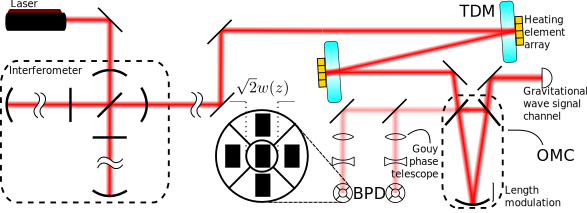
\includegraphics[width=\textwidth]{figs-modematching/blockdiag}
  \end{center}
  \caption[Schematic diagram of the optical layout of a modematching feedback control system.]{Schematic diagram of the optical layout of a modematching feedback control system. Abbreviations are explained in the text. Also shown is the segmentation of the bull's-eye photodetector. The spherical mode mismatch signal combination is A-B-C. The astigmatic signal combination is B-C.}
  \label{fig:mmblockdiag}
\end{figure}
A schematic diagram of the sensing and actuation system is shown in Figure \ref{fig:mmblockdiag}. %NL%
The control system consists of two actuators, two sensors and the resonant optical cavity. %NL%
The actuators are focusing elements with variable focal length; astigmatism control is provided with the ability to induce differing focusing power in the vertical and horizontal directions. %NL%
The laser beam is directed through both actuators and then incident on the input of the cavity. %NL%
The cavity is critically coupled so the correctly matched light is transmitted maximally through the OMC. %NL%
The cavity length is held on resonance by a separate control system. %NL%
The reflected light is directed onto the two mode matching sensors, with Guoy phase telescopes to get good separation of sensed mode quadratures.

\section{Mode matching sensors}
The sensors, are annular segmented photodetectors, also known as bull's-eye photodetectors (BPDs) \cite{Mueller:00}. %NL%
A schematic of the BPD is shown as a part of Figure \ref{fig:mmblockdiag}. %NL%
The mode mismatch is sensed using a heterodyne detection scheme. %NL%
Detection of the bull's-eye mode is done by subtracting the photocurrent of the central segment from those of the outer segments. %NL%


BPDs have been used in a variant of the Pound-Drever-Hall (PDH) scheme where the optical local oscillator was provided by radio frequency (RF) sidebands induced on the input beam by a frontal modulation scheme \cite{Mueller:00}. %NL%
We propose an alternative scheme, using the sidebands induced by length modulation of the cavity for use in a dither servo for length control. %NL%
In Enhanced LIGO, the OMC length modulation frequency was approximately 12kHz. %NL%
These sidebands leak out of the cavity from the reflected port and occupy only the \TEM{00} mode of the cavity. %NL%
This provides a good local oscillator which mixes with the second-order modes due to the segmented photodetector. %NL%
The error signal from the BPD is demodulated at the cavity length modulation frequency which provides a signal proportional to the mixing of the \TEM{00} cavity mode with the rejected second-order modes of the input beam. %NL%
By contrast to PDH, the demodulation occurs at audio frequencies rather than RF.

The signal on the BPD, measured in power at the OMC length modulation frequency, is\cite{Sigg:00,ModalModelUpdate4}
\begin{equation}
\label{eq:signal}
%S = \frac{\sqrt 2 \mathcal{F}}{e \pi} k \delta z P_c \alpha,
S = \frac{1}{\sqrt 2}\left(\frac{2}{e}\right)\left(\frac{2 \mathcal{F}}{\pi}\right)\left(k \delta z\right) P_c \alpha,
\end{equation}
where $e$ the base of the natural logarithm, $k$ is the wave number of the laser light, $\delta z$ is the amplitude of the OMC length modulation, $\mathcal{F}$ is the OMC cavity finesse, $P_c$ is the power in the resonant carrier field incident on the OMC, and $\alpha$ is the ratio of amplitudes of the bull's-eye mode to the \TEM{00} mode incident on the OMC. %NL%
Equation (\ref{eq:signal}) assumes that the sensor is located with the optimal Gouy phase shift for the given mode mismatch.

In Advanced LIGO, the DC optical power on the BPD sensor will likely be dominated by RF sidebands exiting the interferometer which are rejected by the OMC. %NL%
These RF sidebands provide sensing of auxiliary degrees of freedom of the interferometer, but are not relevant for the OMC sensing. %NL%
The shot noise is then
\begin{equation}
N = \sqrt{2 \hbar c k P_{RF}},
\end{equation}
where $P_{RF}$ is the optical power of the RF sidebands, $\hbar$ is the reduced Planck constant, and $c$ is the speed of light in vacuum.

\begin{table}
  \begin{center}
    \begin{tabular}{|r|l|}
      \hline
      Symbol & Value \\
      \hline
      $\mathcal{F}$ &  370\\
      $k$ &  $2\pi/(1064\text{nm})$\\
      $\delta z$ &  $5$pm\\
      $P_c$ &  $100$mW \\
      $P_{RF}$ &  $500$mW \\
      \hline
    \end{tabular}
  \caption{Parameters used to calculate the sensitivity of the BPD.}
  \label{tab:values}
  \end{center}
\end{table}

Using values from Table \ref{tab:values}, we get a shot noise limited SNR of
\begin{equation}
SNR =\frac{S}{N}\sqrt{T}= 8.4\times 10^5 \alpha \sqrt{\frac{T}{1\text{s}}},
\end{equation}
where $T$ is the measurement integration time. %NL%
For a 0.1\perc{} mode mismatch, $\alpha$ takes a value of approximately $0.03$. %NL%
This amount of mode mismatch would have a shot noise limited SNR of $251$ with a $10^{-4}$s integration time. %NL%
This value is sufficiently high that only a fraction of the OMC reflected power will be necessary in practice.

This design would optimize the transmission of the central optical carrier frequency through the OMC. %NL%
In practice, the sensitivity to gravitational-waves depends on the transmission of audio signal sidebands which in principle could occupy differing spatial modes. %NL%
The amount of mismatch of the carrier and audio sidebands that will be present in an interferometer is difficult to predict. %NL%
As discussed in Chapter \ref{ch:beacon}, in the first generation of LIGO, automatic alignment systems were developed which optimally sensed the audio sideband mode because the mismatch proved a problem for traditional alignment systems \cite{Smith-Lefebvre:11,Tobin}. %NL%
Similar mismatch of the bull's-eye mode would contaminate a modematching servo such as that desribed here. %NL%
A solution would involve using the modulation product of the OMC length modulation sidebands with audio sidebands induced in the interferometer arms. %NL%
These induced sidebands are commonly refered to as the beacon sidebands. %NL%
This would give a corresponding reduction of SNR by the modulation depth of the beacon sidebands.

\section{Mode matching actuators}
While Arain et al. %NL%
provide an array of optical elements which can provide a variable focusing power \cite{Arain:10}, for our OMC mode matching servo we propose the use of a design by Canuel et al. %NL%
for use in mode matching control of the Virgo input optics system \cite{Canuel}. %NL%
Canuel et al. %NL%
propose a thermally deformable mirror (TDM) comprising a highly reflective (HR) mirror placed in reverse from the usual orientation, such that the beam passes through the anti-reflective surface and mirror substrate before reflection of the HR surface. %NL%
An array of electronically resistive elements are bonded to the HR surface of the optic. %NL%
Passing current through these resistive elements heats the optic and allows control of the transverse spatial variation of the optical path length, which can be used to induce a thermal lens. %NL%
A fine enough array of elements allows for heating patterns that can control the spherical and astigmatic lens powers separately. %NL%
Canuel et al. %NL%
report on an early prototype made from a BK7 substrate which can provide a variable focusing power with a range of $0.032 \text{m}^{-1} \text{(diopters)}$. %NL%
The design of Canuel et al. %NL%
has certain beneficial features which make it suitable for this application: it is vacuum compatible, it is low noise due to the low thermal time constant, and it is simple to modify existing suspended steering mirror designs to accomodate the heating elements. %NL%
The control bandwidth will be limited by the thermal time constant of these actuators, which should be adequate given that the effects being corrected occur either at thermal time scales or are constant in time.

We may quantify the effect of a perturbation of the focusing power of an optical component by how much of a pure \TEM{00} mode is transferred to the bull's-eye mode for small variations in the focusing power. %NL%
We will assume a system which is well modematched in the absence of pertubation. %NL%
Given an optical element with additional focusing power $d_{\rm mm}$, the resulting mode mismatch amplitude is
\begin{equation}
\label{eq:matrixelement}
U_{\text{bull's-eye}} = -i\frac{k w^2(z)}{4} d_{\rm mm} \times U_{00}\equiv -iDU_{00},
\end{equation}
where $k$ is the wave number of the laser beam, $w(z)$ is the beam width radius measured at the optic position, $U_{00}$ is the \TEM{00} mode amplitude, and $U_{\text{bull's-eye}}$ is the bull's-eye mode amplitude \cite{ModalModelUpdate4}. %NL%
$D$ can be interpreted as the beam-normalized focusing power, with $d_{\rm mm} = (d_v+d_h)/\sqrt{2}$, where $d_h$  and $d_v$ are the focusing powers in the horizontal and vertical directions, respectively. %NL%
To account for the astigmatic mode, one may define $d_{\rm ast}=(d_v-d_h)/\sqrt{2}$ and use a similar equation to that of Equation (\ref{eq:matrixelement}).

The light which is not in the \TEM{00} mode is rejected by the OMC, thus for the regime where $D$ is small, the mode matching efficiency of the OMC is
\begin{equation}
\epsilon \approx 1 - D^2.
\end{equation}
Assuming a design similar to that of Canuel et al. %NL%
can provide 0.05 diopters focusing power, and a beam width radius of 2mm on the mirror, such an actuator would be able to compensate a single quadrature of mode mismatch of up to approximately 10\perc{}. %NL%
It should be noted that the actuation range depends quadratically on the beam size so larger values should be readily achievable.

\section{Chapter summary}
In summary we have provided a conceptual design for a mode matching control system to be used in interferometric gravitational-wave detectors that make use of an OMC. %NL%
We have shown that segmented photodetectors and deformable mirror actuators originally conceived for the controlling mode matching {\it into} the interferometer are also well suited for solving the {\it output }mode matching problem. %NL%
Moreover, we have adapted a modulation scheme designed to control the alignment of the interferometer output mode to the OMC to also yield high SNR mode matching error signals. %NL%
Together, this has allowed us to propose a remotely controllable mode matching servo system. %NL%
The necessity of having such a system was recognized during the commissioning and operation of the Enhanced LIGO detectors, and it will be an important tool for optimizing and maintaining the sensitivity of future gravitational wave detectors, including those of Advanced LIGO and Virgo.

\chapter{Techniques for reducing output mode cleaner beam jitter noise}
%This was in my opinion the most important noise source that came with the inclusion of the OMC in LIGO

% talk about how it was seen by Seiji in 40m cavities, but also by keita with GEO OMC.
\com{Seiji's jitter paper}\cite{Kawamura:94}

\section{The noise mechanism of beam jitter incident on a high finesse cavity}

Motion of the beam incident on a high finesse cavity alters the overlap of said beam with the resonant mode of the cavity. %NL%
This leads to fluctuations in the amount of light which can couple into the cavity and consequently, power fluctuations of the transmitted beam. %NL%
The power fluctuation can spoil the measurement of the intrinsic amplitude modulation of the beam if the measurement and fluctuations occur at the same frequencies.

For a beam incident on the cavity which has a lateral (perpendicular to the direction of propagation) and angular misalignment, constrained to a plane, we have the following expression for the power transmitted through the cavity
\begin{equation}
\label{eqn:simplejitter}
P\approx P_0\left(1-\left(\frac{\Delta x}{w_0}\right)^2-\left(\frac{\theta}{\theta_d}\right)^2\right),
\end{equation}\com{check for factor 2 error, also with modal model chap}
where $P_0$ is the power transmitted of the aligned beam, $\Delta x$ is the beam waist displacement, $\theta$ is the beam waist tilt, $w_0$ is the beam waist radius, and $\theta_d$ is the divergence angle of the beam. %NL%
The approximation holds while both the angular and lateral misalignments are small.

Equation \ref{eqn:simplejitter} shows that beam misalignments couple to the transmitted power quadradically. %NL%
This leads to a few relevant consequences. %NL%
The coupling of beam jitter to transmitted power is nonlinear, thus frequency components of the beam motion may be mixed together, producing new frequencies in the transmitted power. %NL%
Also, the linear coupling coefficient of beam jitter to power fluctuations is proportional to the DC beam misalignment. %NL%
This causes the direct linear coupling of frequency components of beam jitter to power fluctuations to vary as the DC pointing error varies.

Steering optics in the beam path leading to the cavity which are vibrating may transfer vibrations to the laser beam and produce beam jitter noise. %NL%
Let us investigate beam jitter coupling of an optic in the modal picture. %NL%
 We will work in a basis of only the \TEM{00} and \TEM{01} modes. %NL%
Let's assume we have a beam which is dominantly in the \TEM{00} mode as measured in the basis of our cavity, with some small amplitude of \TEM{01} mode. %NL%
In other words, we begin with a beam which is slightly misaligned.
\begin{equation}
\vect{E}_{\text{input}}=E_0\left(\vect{00}+\alpha\vect{01}\right).
\end{equation}
The misalignment, $\alpha$ may be do to another steering mirror upstream, or a misalignment of the beam source relative to our cavity axis, the precise origin is not critical for this discussion.

Now we will assume this beam is incident on a steering mirror before it finally enters the cavity. %NL%
This steering mirror also has a slight misalignment, $\theta$. %NL%
Equation \ref{eqn:mirrortilt} shows the matrix representing the operator of a mirror which has been tilted from nominal alignment. %NL%
The beam incident on the cavity is then
\begin{equation}
\vect{E}_{\text{incident}}=\oper{M}(\Theta)\vect{E}_{\text{input}},
\end{equation}
where, as before, $\Theta=\frac{\theta \pi w(z)}{\lambda}$, while $w(z)$ is the beam width radius at the mirror, and $\lambda$ is the laser wavelength. %NL%
Because the cavity has a high finesse, when the cavity is resonant on the \TEM{00} mode, only that mode is transmitted. %NL%
Thus, for the field transmitted by the cavity
\begin{equation}
E_{\text{t}}=t_{\text{cavity}}\matrixel{00}{\oper{M}\left(\Theta\right)}{E}_{\text{input}}=t_{\text{cavity}}E_0\left(1-i\frac{ \pi w(z)}{\lambda}\theta\alpha\right),
\end{equation}
where \com{finish}. %NL%
This causes a power fluctuation on trasnmission
\begin{equation}
\label{eqn:mirrorjitter}
P=E_t^*E_t=P_0\left(1+\frac{2\pi w(z)}{\lambda}\theta\Im(\alpha)\right).
\end{equation}
Only the imaginary part of $\alpha$ contributes to beam jitter noise of our mirror because it represents an error in alignment \emph{angle}, not position, at the location of the steering mirror $\oper{M}$. %NL%


One interesting consequence of Equation \ref{eqn:mirrorjitter} is that for a given mirror, the strength of beam jitter coupling is proportional to $w(z)$, the size of the beam on the optic. %NL%
Thus one technique for reducing beam jitter coupling is to design one's optical path in such a way that beams are smaller on optics that may produce significant beam jitter. %NL%
This of course also reduces their efficiency as an alignment control mirror.

Futhermore, we again see a nonlinear coupling in the form of mixing of the incident misalignment, $\alpha$, and the jitter of the steering mirror, $\theta$. %NL%
We may suppose that the input alignment has both a DC component and possibly some low frequency (a few to several Hz) wandering motion. %NL%
If this is coupled with high frequency (i.e. %NL%
frequencies in the detection band) jitter of the steering mirror, the mixing of frequencies can cause noise in the power transmission at and around the jitter frequency of the steering optic.

With the introduction of the OMC in Enhanced LIGO, bilinear beamjitter coupling became a much more prominant source of noise. %NL%
Figure \ref{fig:bilinear} shows how low frequency beam motion mixes with high frequency jitter to produce broad sidebands around beam jitter peaks. %NL%
This is similar to how beam jitter was discussed by \citet{Tobin}.

\begin{figure}
  \begin{center}
  \leavevmode
%  \includegraphics{figs-jitter/bilinear.pdf}
  \end{center}
  \caption[add me]{add me}
  \label{fig:bilinear}
\end{figure}

\section{Mechanical resonances of beam steering optics}
When the Enhanced LIGO interferometers were first performing at a sensitivity comparable to the state of the interferometers in the S5 science run, there were large glaring peaks in the sensitivity spectrum. %NL%
It was determined fairly quickly that these were due beam jitter, but the mechanism causing the jitter was unkown.

The Enhanced LIGO upgrade introduced several modifications to the readout chain of the interferometer. %NL%
As discussed in Chapter \ref{ch:omc}, with the introduction of the in-vacuum OMC, it was necessary to use new beam steering and modematching optics to couple the beam exiting the interferometer to the OMC cavity. %NL%
These steering optics, as well as the OMC, were all housed in a single vacuum chamber on top of the prototype HAM ISI platform which is planned to be used copiously in Advanced LIGO. %NL%
Although it was not fully appreciated at the start of Enhanced LIGO, the new isolation platform provided much reduced vibration isolation at audio frequencies when compared to the isolation tables used in the HAM chambers in Initial LIGO. %NL%
Figure \ref{fig:hamtransmission} shows a comparison of the transmission of ground motion to motion of the HAM table for both the initial LIGO passive isolation system, and the Enhanced LIGO HAM ISI.

\begin{figure}
  \begin{center}
  \leavevmode
  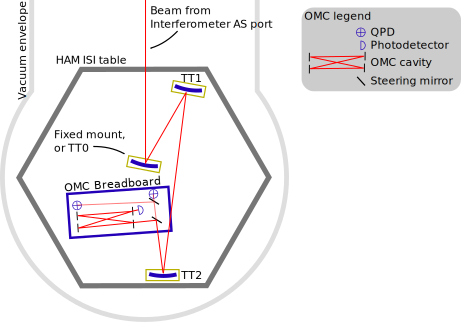
\includegraphics{figs-jitter/ham6layout.pdf}
  \end{center}
  \caption[add me]{add me \com{don't forget QPDs}}
  \label{fig:ham6layout}
\end{figure}

\begin{figure}
  \begin{center}
  \leavevmode
  \includegraphics{figs-jitter/hamtransmission.pdf}
  \end{center}
  \caption[add me]{add me. The high frequency behavior of the HAM ISI model (green curve) represents true resonant structure and is not attributed to measurement noise. Credit and appreciation for this figure goes to Jeff Kissel.}
  \label{fig:hamtransmission}
\end{figure}

The optical layout of the OMC chamber of Enhanced LIGO comprised three steering optics, which also behaved as a mode matching telescope, and the OMC itself. %NL%
In the initial configuration, the first of these was a mirror on a fixed mount, while the other two were in a Tip-Tilt suspension system with active beam steering. %NL%
A diagram of the optical layout is shown in Figure \ref{fig:ham6layout}. %NL%
Diligent work by Robert Schofield determined that some of the largest beam jitter peaks degrading the interferometer sensitivity were due to vibrations of the fixed mirror mount.\com{citation? %NL%
elog?} To rectify this situations, the fixed mirror mount was replaced with a small mirror suspension similar to the Tip Tilts but without the active steering control. %NL%
Comparison of the old and new designs are shown in Figure \ref{fig:TT0photos}. %NL%
This new style was refered to as the passive Tip Tilt, or TT0. %NL%
As seen in Figure \ref{sensimprovement}, this was effective at removing the largest peaks, though some new peaks appeared \com{somewhere}.

\begin{figure}
  \begin{center}
  \leavevmode
%  \includegraphics{figs-jitter/TT0photos.pdf}
  \end{center}
  \caption[add me]{add me}
  \label{fig:TT0photos}
\end{figure}

The origin of the peaks located in the most sensitive region of the LIGO sensitivity spectrum (``the bucket'') was finally determined by a measurement of the coupling of motion from the table to the pointing of the laser beam itself. %NL%
The OMC was equipped with a pair of quadrant photodetectors (QPDs) which sampled the beam incident on the OMC. %NL%
These QPDs were used to measure the response of the beam motion to motion of the ISI table, which is measured by inertial sensors built into the table. %NL%
A measurement of the transfer function of table motion to beam motion may be seen in Figure \ref{fig:TTbounceTF}. %NL%
The resonances were determined to be the vertical bounce mode of the optic in the suspension. %NL%
\com{justify}

\begin{figure}
  \begin{center}
  \leavevmode
%  \includegraphics{figs-jitter/TT0photos.pdf}
  \end{center}
  \caption[add me]{add me}
  \label{fig:TTbounceTF}
\end{figure}

The Tip Tilt design had originally assumed the vertical restoring force was due only to strethcing tension in the wires. %NL%
The vertical resonance was expected to lie near the 340Hz violin resonances of the main interferometer test mass suspensions, which were already In fact, the wires had a sufficient gague of \com{big} which caused the break off point of the suspension to be far from the wire clamp. %NL%
This resulted in the wire taking more of an `S' shape than expected, as shown in Figure \ref{fig:ttdiag}. %NL%
The bend in the wire resulted in giving the wire much more yield, reducing the resonant frequencies and placing them directly in the most sensitive region of LIGO. %NL%
\com{maybe talk about matt's fea model.} 

\begin{figure}
  \begin{center}
  \leavevmode
  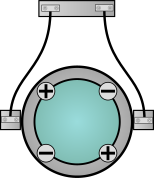
\includegraphics{figs-jitter/ttdiag.pdf}
  \end{center}
  \caption[add me]{add me}
  \label{fig:ttdiag}
\end{figure}

The Tip Tilt suspension was first modified by using thinner wires of gague \com{small}. %NL%
This had the desired effect of reducing the frequency of the bounce resonance to be below the sensitive measurement band, but could not function as a permanent solution due to the fragility of the wires.\footnote{One of the Tip Tilts doubled as a fast beam diverter to protect the OMC photodiodes from the full stored energy of the arm cavities which exits the AS port when the interferometer loses lock. %NL%
This system would put considerable force on the suspension and after several lock loss cycles it broke one of the Tip Tilt suspension wires.} The ultimate solution was to place the upper wire clamps at the ends of blade springs. %NL%
The new Tip Tilt assembly is shown in Figure \ref{fig:bladephoto}. %NL%
This reduced the vertical resonances to \com{something Hz}, outside of the sensitive region, but while still allowing the use of wires with enough strength. %NL%
The sensitivity of the interferometer after this change was made is shown in Figure \ref{fig:sensimprovement}.

\begin{figure}
  \begin{center}
  \leavevmode
%  \includegraphics{figs-jitter/hamtransmission.pdf}
  \end{center}
  \caption[add me]{add me.}
  \label{fig:bladephoto}
\end{figure}

\begin{figure}
  \begin{center}
  \leavevmode
%  \includegraphics{figs-jitter/hamtransmission.pdf}
  \end{center}
  \caption[add me]{add me.}
  \label{fig:sensimprovement}
\end{figure}

Mechanical resonances of optic supports in the beam path should stay in the front of the mind of those investigating sources of beam jitter noise. %NL%
Determining the precise source is certainly helped by having the luxury of an optics table equipped with position sensors and an actuation system.
\section{Magnetic field coupling and feedforward subtraction}
Even after the mitigation of mechanical beam jitter on the OMC, there was still significant pollution of the LIGO sensitivity at frequencies surrounding 60Hz. %NL%
60Hz is the frequency of the AC power distribution system in the U.S.A. %NL%
and is a well known source of trouble to those attempting to do precision measurement. %NL%
It is not terribly troublesome if 60Hz interference into one's device is fairly narrow-band. %NL%
During Enhanced LIGO comissioning however, the 60Hz line was surrounded by broad sidebands which were infered to be caused by beam jitter. %NL%
This was particularly troubling because of the importance of sensitivity to gravitational wave emission from the Crab pulsar, which is expected to emit gravitational waves at 59.56Hz \cite{Crab}.

The Tip Tilt suspensions utilized permanent magnets affixed to the optics and coil electromagnets for active beam steering control. %NL%
The four permanent magnets were arranged on the face of the optic as shown in Figure \ref{fig:ttdiag}. %NL%
The polarities were alternated so that uniform ambient magnetic fields would not cause a force or torque on the optic. %NL%
Robert Schofield determined that the source of the beam jitter peaks at multiples of 60Hz were in fact due to \emph{gradients} in the ambient magnetic field at those frequencies. %NL%
He also suggested that the use of a magnetometer sensor outside of the vacuum chamber would provide a signal that could be applied to the Tip Tilt alignment control and cancel the effects of the ambient field.\com{cite robert's elog} In addition, the strength of the permanent dipole magnets used in the Tip Tilts was reduced.

A magnetometer was installed and a feedforward control system was implemented in the LIGO realtime system for digital signal processing. %NL%
The feedforward system read the digitized 3-axis magnetometer signal, performed filtering, and fed the filtered signal to the Tip Tilt pitch and yaw actuators. %NL%
A diagram of the system may be seen in Figure \ref{fig:magffblockdiag}. %NL%


\begin{figure}
  \begin{center}
  \leavevmode
  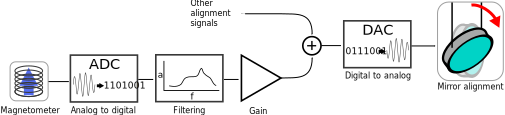
\includegraphics{figs-jitter/magffblockdiag.pdf}
  \end{center}
  \caption[add me]{add me}
  \label{fig:magffblockdiag}
\end{figure}

To reduce the 60Hz jitter peak, the signal filtering was tuned to minimize the presence of 60Hz motion measured by the OMC QPDs. %NL%
When correctly tuned, the feedforward system was able to significantly reduce the magnitude of the sidebands around 60Hz in the LIGO sensitivity spectrum. %NL%
\com{performance figure}

Such a feedforward servo is beneficial whenever one has a signal which is coherent with the source of high frequency jitter noise. %NL%
Because of the bilinear coupling of beam jitter, removal of even narrow, single frequency, components of beam motion can reduce broadband sources of noise in one's data. %NL%
With only the magnetometer signal, it would not be possible to perform off-line subtraction of the sidebands around 60Hz from the final data stream. %NL%
However, it has been shown \com{by sergei et al} that it is possible to combine several signals, in a nonlinear way, to subtract sources of bilinear-coupled noise from off-line data.\com{citation} This rather impressive technique has already been shown to be well suited for reduction of beam jitter noise.

\section{The relationship of alignment control and beam jitter}
% depending on bandwidth, alignment system can remove low/DC or high. Though not if you are using a beacon system. Also beware of fringe wrapping.
As discussed in Chapter \ref{ch:beacon}, a standard cavity alignment control system is designed to minimize the \TEM{01} and \TEM{10} mode content incident on the cavity. %NL%
We have also just seen that any misalignment increases the linear coupling of beam jitter noise to the cavity transmission signal. %NL%
This connection is manifestly clear in the case of a dither alignment servo, where beam jitter is purposely induced on the beam, and the servo obtains optimum alignment by minimizing the coupling of the dither frequency in transmission. %NL%
If the DC and low frequencies of the alignment error can be sufficiently supressed by a control system, the beam jitter coupling is consequently reduced.

%Attempts were made in Enhanced LIGO to directly reduce the high frequency beam jitter on the OMC with a high bandwidth alignment servo. For sufficiently high control bandwith, it was seen that an increase in gain would cause an increase in broadband noise in the OMC transmission. One possible mechanism for the increased noise \com{OMC backscatter} \cite{T060303}.

We break this relationship between alignment optimization and jitter coupling minimization when a beacon or optimal style alignment system is used as desribed in Section \ref{sec:beaconalignment}. %NL%
Because the carrier frequency component is often the dominant contribution to the total power of the transmitted signal, it is usually the case that beam jitter noise orignating from the carrier is dominant over other frequency components. %NL%
Alignment schemes which optimize the alignment of the audio frequency signal sidebands will disregard the HOM content of the carrier beam, and thus may increase beam jitter coupling. %NL%
This additional beam jitter coupling may be mitigated by control of the relative modal content of the audio sidebands and the carrier, which will be discussed in the following section.

\section[Modification of the relative modal content of the carrier and audio sidebands]{Modification of the relative modal content of the carrier and audio sidebands\footnote{This section will satisfy as mearly a record of some lore learned during Enhanced LIGO. It is not intended to provide a quantitative model, but merely act as a guide for future efforts.}}

After the implementation of the beacon alignment system in Enhanced LIGO, some beam jitter peaks of unknown origin remained in the sensitive region of the detector. %NL%
\com{figure?}. %NL%
It was discovered that the height of these peaks were controlable by modifying the beam position on the antisymmetric port alignment sensor\footnote{In Initial/Enhanced LIGO, this was known as WFS1.} of the main interferometer alignment control system. %NL%
We postulated that because of offsets in the readout of the interferometer alignment signals, changing the beam position would change the error point offsets of the alignment feedback system of the main interferometer. %NL%
The antisymmetric port signal primarily feeds back to the differential alignment mode of the ETMs. %NL%
It was thought that this lead to a redistribution of the modal content of the carrier field exiting the antisymetric port of the interferometer relative to the fields of the audio sidebands. %NL%
One could imagine that the position of a local minimum, with respect to alignment, of the carrier transmission could be moved into coincidence with the optimal alignment point of the signal fields. %NL%
Attempts were made to instead directly inject offsets into the alignment error signals to produce the same effect, but they were never as successful as varying the pointing on the alingment sensor.

\chapter{Conclusion}
\label{ch:conclusion}

OMC betterness
\com{aLIGO OMC design \cite{T1000276} changes \cite{T0900157}}

beacon betterness
\com{stable cavities \cite{T080208}}

Mode matching betterness
\com{Mode matching Chapter \ref{ch:modematching}}

Beam jitter betterness
\com{aLIGO TT design \cite{slagmolen:12}}
\com{quad design \cite{quaddesign}}


\appendix

\chapter{Practical calculations using matrices based on the optical vector space model}
%%% Local Variables: 
%%% mode: latex
%%% TeX-master: "main"
%%% End: 

\chapter{Additional notes}

\section{Conventions for the coefficient of amplitude transmission and reflectivity of beamsplitters}

\section{Dither sensing is a measurement of a partial derivative}

%%% Local Variables: 
%%% mode: latex
%%% TeX-master: "main"
%%% End: 

\chapter{Common misconceptions about laser interferometer gravitational-wave antennae}

\section{The sensitivity/bandwidth ``tradeoff''}
There is an argument that exists in various places in the literature when considering the response of the Fabry-Perot resonant arm cavities of a gravitational wave antenna. %NL%
The argument goes something like this:
\begin{itemize}
\item When designing an interferometer, one must choose the finesse of the arm cavities.
\item An increase in the finesse leads to an increase of stored power in the arms, which increases the sensitivity to gravitational waves.
\item The finesse also negatively impacts the bandwidth of the arm cavities. An increase in finesse leads to a reduction in sensitivity to gravitational waves at frequencies higher than the cavity bandwidth.
\item Thus there is a tradeoff between senitivity and bandwidth, and one must choose the arm cavity finesse to balance the benefits of each.
\end{itemize}

Noise sources that are frequency independant (white) at the photodetector will have a frequency dependent structure shaped as the inverse of the interferometer optical sensitivity. %NL%
In other words, as the interferometer sensitivity decreases, the contribution from that noise source to limiting the ultimate measurement correspondingly increases. %NL%
So sometimes the above argument is given in terms of the shape of the shot noise contribution (which is white at the photodetector) of the interferometer. %NL%
In that case, the argument might say that an interferometer with a higher finesse will have a lower cavity pole, and hence, the shot noise will begin rising in frequency earlier, ultimately leading to a higher noise floor at high frequencies.

The flaw in the argument arises when one actually compares the effects of the two competing contibutions to the interferometer sensitivity. %NL%
This is well illustrated by considering the shot noise floor of a Michelson Interferometer with Fabry Perot arms (FPMI). %NL%
The amplitude spectral density of shot noise of this interferometer, calibrated as refered to the strain measured by the interferometer is \cite{LIGO}
\begin{equation}
\label{eqn:FPMIshotnoise}
h_{\rm{shot}}^{\rm{FPMI}}=\sqrt{\frac{\pi \hbar \lambda}{c P_{\rm{BS}}}}\left(\frac{\sqrt{1+(4 \pi\tau f)^2}}{4 \pi \tau }\right)=h_{\rm{shot}}^{\rm{MI}}\times \frac{\pi\sqrt{1+(4\mathcal{F})^2(f/\rm{FSR})^2}}{2 \mathcal{F}},
\end{equation}
where $\hbar$ is the reduced Planck constant, $\lambda$ is the laser wavelength, $c$ is the speed of light, $P_{\rm{BS}}$ is the light incident on the beam splitter, $\tau=\frac{\mathcal{F}}{\pi \rm{FSR}}$ is the light storage time of the arm cavities, $\rm{FSR}$ is the cavity free spectral range, and $\mathcal{F}$ is the cavity finesse. %NL%
The second equality shows the shot noise scaled by the shot noise in a Michelson interferometer with no cavity arms. %NL%
Equation \ref{eqn:FPMIshotnoise} shows how the behavior of the sensitivity of the interferometer depends on the cavity finesse. %NL%
The low frequency sensitivity is indeed improved with an increased finesse, the shot noise decreses. %NL%
However at high frequencies, where $f \gg \rm{FSR}/4\mathcal{F}$, the effect of the finesse cancels out, and an increase in finesse does not reduce the sensitivity of the interferometer. %NL%
Figure \ref{fig:fpmishotnoise} shows how the shot noise sensitivity changes as a result of changing the arm cavity finesse. %NL%
As one can see, the high frequency sensitivities are all the same. %NL%
So there is no trade-off, an increase in finesse can only benefit the sensitivity, at least in this simplified case.\footnote{This no longer is true, for example, when losses are included.}

\begin{figure}
  \begin{center}
  \leavevmode
  \includegraphics{figs-ap-miscon/fpmishotnoise.pdf}
  \end{center}
  \caption[]{}
  \label{fig:fpmishotnoise}
\end{figure}

In reality, there are good reasons to limit the finesse of the arm cavities. %NL%
These include difficulty of lock acuisition, the ability to deal with very large amounts of stored power in the arm, and the fact that the loss experienced in one round trip through the arm is multiplied by the number of bounces the light experiences.

The choice of the arm cavity finesse for a FPMI is usually driven by the existence of other noise sources. %NL%
The finesse can be increased until other, low frequency, noise sources dominate and there is no benefit to increase the finesse further.

In the case of a FPMI, the finesse governs both the stored arm power and the bandwidth of the differential mode interferometer, or the recycling of the gravitational wave audio sidebands. %NL%
The addition of a signal recycling/extraction mirror, as in Advanced LIGO, breaks this symmetry. %NL%
The signal mirror can be used to modify the detector bandwidth, without changing the stored arm cavity power.

The author is not certain about where this misconception comes from. %NL%
For example, it is treated correctly in the classic reference by \citet{saulson1994fundamentals}. %NL%
On page 103, about the high frequency regime, he writes, ``Further increase in the finesse of the arm cavities neither helps, nor in this simple case hurts, the sensitivity.''

\section{Why LIGO has two arms}
This misconception is alluded to in Section \ref{sec:michelson}, but is treated here more directly. %NL%
People who are knowledgeable about LIGO, but are not familiar with the details of the interferometer are often surprised to learn that the main reasons driving the use of a Michelson interferometer, with two long arms, are related to the coupling of technical noise sources, and not because of the fact that gravitational waves stretch along perpendicular axes.

A Michelson interferometer with symmetric arms bestows the experimentalist with the powerful gift of \emph{common mode noise rejection}. %NL%
Technical fluctuations of the laser amplitude and frequency tend to reflect back to the laser, not to the dark fringe of the Michelson. %NL%
The added benefit of the common mode servo (Section \ref{sec:armcav}) also can be used to reduce the laser frequency noise. %NL%
Again, this is treated beautifully in Sections 10.1.4 and 12.6 of \citet{saulson1994fundamentals}. %NL%


A two-armed interferometer is a significant increase in complexity, though the signal strength is only two times that of a one-armed interferometer. %NL%
It is the massive reduction of noise that makes the complexity worthwile.

\section{With a DARM offset, is LIGO still a null measurement?}
This is not a misconception {\it per se}, but is an intersting point that deserves a small bit of discussion.

\chapter{Abbreviation glossary}

\begin{nicgloss}
  \item[First] The first item
  \item[Second] The second item
  \item[Third] The third etc \ldots
\end{nicgloss}


\rfoot{}
\input{biblio}

\end{document}

